%\documentclass{standalone}
%\usepackage{tikz}
%\usetikzlibrary{patterns,plotmarks}
%\begin{document}
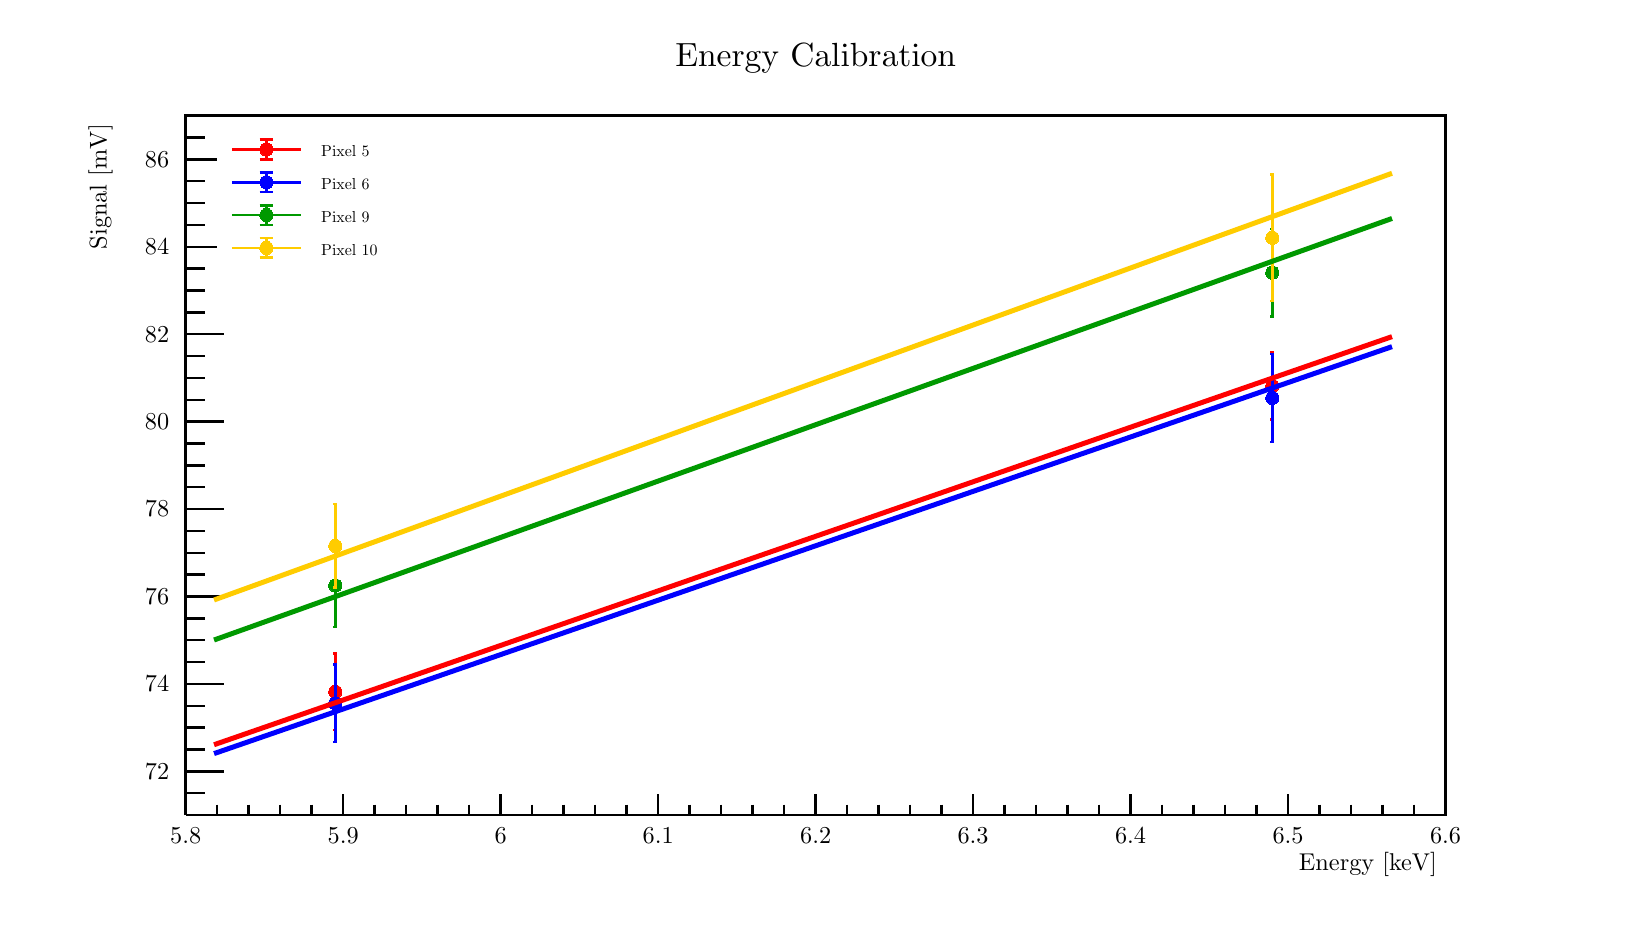
\begin{tikzpicture}
\def\CheckTikzLibraryLoaded#1{ \ifcsname tikz@library@#1@loaded\endcsname \else \PackageWarning{tikz}{usetikzlibrary{#1} is missing in the preamble.} \fi }
\CheckTikzLibraryLoaded{patterns}
\CheckTikzLibraryLoaded{plotmarks}
\pgfdeclareplotmark{cross} {
\pgfpathmoveto{\pgfpoint{-0.3\pgfplotmarksize}{\pgfplotmarksize}}
\pgfpathlineto{\pgfpoint{+0.3\pgfplotmarksize}{\pgfplotmarksize}}
\pgfpathlineto{\pgfpoint{+0.3\pgfplotmarksize}{0.3\pgfplotmarksize}}
\pgfpathlineto{\pgfpoint{+1\pgfplotmarksize}{0.3\pgfplotmarksize}}
\pgfpathlineto{\pgfpoint{+1\pgfplotmarksize}{-0.3\pgfplotmarksize}}
\pgfpathlineto{\pgfpoint{+0.3\pgfplotmarksize}{-0.3\pgfplotmarksize}}
\pgfpathlineto{\pgfpoint{+0.3\pgfplotmarksize}{-1.\pgfplotmarksize}}
\pgfpathlineto{\pgfpoint{-0.3\pgfplotmarksize}{-1.\pgfplotmarksize}}
\pgfpathlineto{\pgfpoint{-0.3\pgfplotmarksize}{-0.3\pgfplotmarksize}}
\pgfpathlineto{\pgfpoint{-1.\pgfplotmarksize}{-0.3\pgfplotmarksize}}
\pgfpathlineto{\pgfpoint{-1.\pgfplotmarksize}{0.3\pgfplotmarksize}}
\pgfpathlineto{\pgfpoint{-0.3\pgfplotmarksize}{0.3\pgfplotmarksize}}
\pgfpathclose
\pgfusepathqstroke
}
\pgfdeclareplotmark{cross*} {
\pgfpathmoveto{\pgfpoint{-0.3\pgfplotmarksize}{\pgfplotmarksize}}
\pgfpathlineto{\pgfpoint{+0.3\pgfplotmarksize}{\pgfplotmarksize}}
\pgfpathlineto{\pgfpoint{+0.3\pgfplotmarksize}{0.3\pgfplotmarksize}}
\pgfpathlineto{\pgfpoint{+1\pgfplotmarksize}{0.3\pgfplotmarksize}}
\pgfpathlineto{\pgfpoint{+1\pgfplotmarksize}{-0.3\pgfplotmarksize}}
\pgfpathlineto{\pgfpoint{+0.3\pgfplotmarksize}{-0.3\pgfplotmarksize}}
\pgfpathlineto{\pgfpoint{+0.3\pgfplotmarksize}{-1.\pgfplotmarksize}}
\pgfpathlineto{\pgfpoint{-0.3\pgfplotmarksize}{-1.\pgfplotmarksize}}
\pgfpathlineto{\pgfpoint{-0.3\pgfplotmarksize}{-0.3\pgfplotmarksize}}
\pgfpathlineto{\pgfpoint{-1.\pgfplotmarksize}{-0.3\pgfplotmarksize}}
\pgfpathlineto{\pgfpoint{-1.\pgfplotmarksize}{0.3\pgfplotmarksize}}
\pgfpathlineto{\pgfpoint{-0.3\pgfplotmarksize}{0.3\pgfplotmarksize}}
\pgfpathclose
\pgfusepathqfillstroke
}
\pgfdeclareplotmark{newstar} {
\pgfpathmoveto{\pgfqpoint{0pt}{\pgfplotmarksize}}
\pgfpathlineto{\pgfqpointpolar{44}{0.5\pgfplotmarksize}}
\pgfpathlineto{\pgfqpointpolar{18}{\pgfplotmarksize}}
\pgfpathlineto{\pgfqpointpolar{-20}{0.5\pgfplotmarksize}}
\pgfpathlineto{\pgfqpointpolar{-54}{\pgfplotmarksize}}
\pgfpathlineto{\pgfqpointpolar{-90}{0.5\pgfplotmarksize}}
\pgfpathlineto{\pgfqpointpolar{234}{\pgfplotmarksize}}
\pgfpathlineto{\pgfqpointpolar{198}{0.5\pgfplotmarksize}}
\pgfpathlineto{\pgfqpointpolar{162}{\pgfplotmarksize}}
\pgfpathlineto{\pgfqpointpolar{134}{0.5\pgfplotmarksize}}
\pgfpathclose
\pgfusepathqstroke
}
\pgfdeclareplotmark{newstar*} {
\pgfpathmoveto{\pgfqpoint{0pt}{\pgfplotmarksize}}
\pgfpathlineto{\pgfqpointpolar{44}{0.5\pgfplotmarksize}}
\pgfpathlineto{\pgfqpointpolar{18}{\pgfplotmarksize}}
\pgfpathlineto{\pgfqpointpolar{-20}{0.5\pgfplotmarksize}}
\pgfpathlineto{\pgfqpointpolar{-54}{\pgfplotmarksize}}
\pgfpathlineto{\pgfqpointpolar{-90}{0.5\pgfplotmarksize}}
\pgfpathlineto{\pgfqpointpolar{234}{\pgfplotmarksize}}
\pgfpathlineto{\pgfqpointpolar{198}{0.5\pgfplotmarksize}}
\pgfpathlineto{\pgfqpointpolar{162}{\pgfplotmarksize}}
\pgfpathlineto{\pgfqpointpolar{134}{0.5\pgfplotmarksize}}
\pgfpathclose
\pgfusepathqfillstroke
}
\definecolor{c}{rgb}{1,1,1};
\draw [color=c, fill=c] (0,0) rectangle (20,11.1035);
\draw [color=c, fill=c] (2,1.11035) rectangle (18,9.99319);
\definecolor{c}{rgb}{0,0,0};
\draw [c,line width=0.9] (2,1.11035) -- (2,9.99319) -- (18,9.99319) -- (18,1.11035) -- (2,1.11035);
\definecolor{c}{rgb}{1,1,1};
\draw [color=c, fill=c] (2,1.11035) rectangle (18,9.99319);
\definecolor{c}{rgb}{0,0,0};
\draw [c,line width=0.9] (2,1.11035) -- (2,9.99319) -- (18,9.99319) -- (18,1.11035) -- (2,1.11035);
\draw [c,line width=0.9] (2,1.11035) -- (18,1.11035);
\draw [c,line width=0.9] (2,1.37684) -- (2,1.11035);
\draw [c,line width=0.9] (2.4,1.2436) -- (2.4,1.11035);
\draw [c,line width=0.9] (2.8,1.2436) -- (2.8,1.11035);
\draw [c,line width=0.9] (3.2,1.2436) -- (3.2,1.11035);
\draw [c,line width=0.9] (3.6,1.2436) -- (3.6,1.11035);
\draw [c,line width=0.9] (4,1.37684) -- (4,1.11035);
\draw [c,line width=0.9] (4.4,1.2436) -- (4.4,1.11035);
\draw [c,line width=0.9] (4.8,1.2436) -- (4.8,1.11035);
\draw [c,line width=0.9] (5.2,1.2436) -- (5.2,1.11035);
\draw [c,line width=0.9] (5.6,1.2436) -- (5.6,1.11035);
\draw [c,line width=0.9] (6,1.37684) -- (6,1.11035);
\draw [c,line width=0.9] (6.4,1.2436) -- (6.4,1.11035);
\draw [c,line width=0.9] (6.8,1.2436) -- (6.8,1.11035);
\draw [c,line width=0.9] (7.2,1.2436) -- (7.2,1.11035);
\draw [c,line width=0.9] (7.6,1.2436) -- (7.6,1.11035);
\draw [c,line width=0.9] (8,1.37684) -- (8,1.11035);
\draw [c,line width=0.9] (8.4,1.2436) -- (8.4,1.11035);
\draw [c,line width=0.9] (8.8,1.2436) -- (8.8,1.11035);
\draw [c,line width=0.9] (9.2,1.2436) -- (9.2,1.11035);
\draw [c,line width=0.9] (9.6,1.2436) -- (9.6,1.11035);
\draw [c,line width=0.9] (10,1.37684) -- (10,1.11035);
\draw [c,line width=0.9] (10.4,1.2436) -- (10.4,1.11035);
\draw [c,line width=0.9] (10.8,1.2436) -- (10.8,1.11035);
\draw [c,line width=0.9] (11.2,1.2436) -- (11.2,1.11035);
\draw [c,line width=0.9] (11.6,1.2436) -- (11.6,1.11035);
\draw [c,line width=0.9] (12,1.37684) -- (12,1.11035);
\draw [c,line width=0.9] (12.4,1.2436) -- (12.4,1.11035);
\draw [c,line width=0.9] (12.8,1.2436) -- (12.8,1.11035);
\draw [c,line width=0.9] (13.2,1.2436) -- (13.2,1.11035);
\draw [c,line width=0.9] (13.6,1.2436) -- (13.6,1.11035);
\draw [c,line width=0.9] (14,1.37684) -- (14,1.11035);
\draw [c,line width=0.9] (14.4,1.2436) -- (14.4,1.11035);
\draw [c,line width=0.9] (14.8,1.2436) -- (14.8,1.11035);
\draw [c,line width=0.9] (15.2,1.2436) -- (15.2,1.11035);
\draw [c,line width=0.9] (15.6,1.2436) -- (15.6,1.11035);
\draw [c,line width=0.9] (16,1.37684) -- (16,1.11035);
\draw [c,line width=0.9] (16.4,1.2436) -- (16.4,1.11035);
\draw [c,line width=0.9] (16.8,1.2436) -- (16.8,1.11035);
\draw [c,line width=0.9] (17.2,1.2436) -- (17.2,1.11035);
\draw [c,line width=0.9] (17.6,1.2436) -- (17.6,1.11035);
\draw [c,line width=0.9] (18,1.37684) -- (18,1.11035);
\draw [anchor=base] (2,0.743937) node[scale=0.877495, color=c, rotate=0]{5.8};
\draw [anchor=base] (4,0.743937) node[scale=0.877495, color=c, rotate=0]{5.9};
\draw [anchor=base] (6,0.743937) node[scale=0.877495, color=c, rotate=0]{6};
\draw [anchor=base] (8,0.743937) node[scale=0.877495, color=c, rotate=0]{6.1};
\draw [anchor=base] (10,0.743937) node[scale=0.877495, color=c, rotate=0]{6.2};
\draw [anchor=base] (12,0.743937) node[scale=0.877495, color=c, rotate=0]{6.3};
\draw [anchor=base] (14,0.743937) node[scale=0.877495, color=c, rotate=0]{6.4};
\draw [anchor=base] (16,0.743937) node[scale=0.877495, color=c, rotate=0]{6.5};
\draw [anchor=base] (18,0.743937) node[scale=0.877495, color=c, rotate=0]{6.6};
\draw [anchor= east] (18,0.488556) node[scale=0.877495, color=c, rotate=0]{Energy [keV]};
\draw [c,line width=0.9] (2,1.11035) -- (2,9.99319);
\draw [c,line width=0.9] (2.48,1.66553) -- (2,1.66553);
\draw [c,line width=0.9] (2.24,1.94312) -- (2,1.94312);
\draw [c,line width=0.9] (2.24,2.22071) -- (2,2.22071);
\draw [c,line width=0.9] (2.24,2.4983) -- (2,2.4983);
\draw [c,line width=0.9] (2.48,2.77589) -- (2,2.77589);
\draw [c,line width=0.9] (2.24,3.05347) -- (2,3.05347);
\draw [c,line width=0.9] (2.24,3.33106) -- (2,3.33106);
\draw [c,line width=0.9] (2.24,3.60865) -- (2,3.60865);
\draw [c,line width=0.9] (2.48,3.88624) -- (2,3.88624);
\draw [c,line width=0.9] (2.24,4.16383) -- (2,4.16383);
\draw [c,line width=0.9] (2.24,4.44142) -- (2,4.44142);
\draw [c,line width=0.9] (2.24,4.71901) -- (2,4.71901);
\draw [c,line width=0.9] (2.48,4.99659) -- (2,4.99659);
\draw [c,line width=0.9] (2.24,5.27418) -- (2,5.27418);
\draw [c,line width=0.9] (2.24,5.55177) -- (2,5.55177);
\draw [c,line width=0.9] (2.24,5.82936) -- (2,5.82936);
\draw [c,line width=0.9] (2.48,6.10695) -- (2,6.10695);
\draw [c,line width=0.9] (2.24,6.38454) -- (2,6.38454);
\draw [c,line width=0.9] (2.24,6.66213) -- (2,6.66213);
\draw [c,line width=0.9] (2.24,6.93971) -- (2,6.93971);
\draw [c,line width=0.9] (2.48,7.2173) -- (2,7.2173);
\draw [c,line width=0.9] (2.24,7.49489) -- (2,7.49489);
\draw [c,line width=0.9] (2.24,7.77248) -- (2,7.77248);
\draw [c,line width=0.9] (2.24,8.05007) -- (2,8.05007);
\draw [c,line width=0.9] (2.48,8.32766) -- (2,8.32766);
\draw [c,line width=0.9] (2.24,8.60525) -- (2,8.60525);
\draw [c,line width=0.9] (2.24,8.88283) -- (2,8.88283);
\draw [c,line width=0.9] (2.24,9.16042) -- (2,9.16042);
\draw [c,line width=0.9] (2.48,9.43801) -- (2,9.43801);
\draw [c,line width=0.9] (2.24,1.38794) -- (2,1.38794);
\draw [c,line width=0.9] (2.24,1.11035) -- (2,1.11035);
\draw [c,line width=0.9] (2.24,9.7156) -- (2,9.7156);
\draw [c,line width=0.9] (2.24,9.99319) -- (2,9.99319);
\draw [anchor= east] (1.9,1.66553) node[scale=0.877495, color=c, rotate=0]{72};
\draw [anchor= east] (1.9,2.77589) node[scale=0.877495, color=c, rotate=0]{74};
\draw [anchor= east] (1.9,3.88624) node[scale=0.877495, color=c, rotate=0]{76};
\draw [anchor= east] (1.9,4.99659) node[scale=0.877495, color=c, rotate=0]{78};
\draw [anchor= east] (1.9,6.10695) node[scale=0.877495, color=c, rotate=0]{80};
\draw [anchor= east] (1.9,7.2173) node[scale=0.877495, color=c, rotate=0]{82};
\draw [anchor= east] (1.9,8.32766) node[scale=0.877495, color=c, rotate=0]{84};
\draw [anchor= east] (1.9,9.43801) node[scale=0.877495, color=c, rotate=0]{86};
\draw [anchor= east] (0.918529,9.99319) node[scale=0.877495, color=c, rotate=90]{Signal [mV]};
\definecolor{c}{rgb}{1,0,0};
\draw [c,line width=0.9] (3.9,2.73079) -- (3.9,3.16206);
\draw [c,line width=0.9] (3.9,2.6218) -- (3.9,2.19053);
\draw [c,line width=0.9] (3.87275,3.16206) -- (3.92725,3.16206);
\draw [c,line width=0.9] (3.87275,2.19053) -- (3.92725,2.19053);
\draw [c,line width=0.9] (15.8,6.61621) -- (15.8,6.99053);
\draw [c,line width=0.9] (15.8,6.50722) -- (15.8,6.13291);
\draw [c,line width=0.9] (15.7728,6.99053) -- (15.8272,6.99053);
\draw [c,line width=0.9] (15.7728,6.13291) -- (15.8272,6.13291);
\foreach \P in {(3.9,2.67629), (15.8,6.56172)}{\draw[mark options={color=c,fill=c},mark size=2.402402pt, line width=0.000000pt, mark=*] plot coordinates {\P};}
\definecolor{c}{rgb}{0,0,1};
\draw [c,line width=0.9] (3.9,2.58478) -- (3.9,3.02319);
\draw [c,line width=0.9] (3.9,2.47579) -- (3.9,2.03737);
\draw [c,line width=0.9] (3.87275,3.02319) -- (3.92725,3.02319);
\draw [c,line width=0.9] (3.87275,2.03737) -- (3.92725,2.03737);
\draw [c,line width=0.9] (15.8,6.46301) -- (15.8,6.96896);
\draw [c,line width=0.9] (15.8,6.35402) -- (15.8,5.84806);
\draw [c,line width=0.9] (15.7728,6.96896) -- (15.8272,6.96896);
\draw [c,line width=0.9] (15.7728,5.84806) -- (15.8272,5.84806);
\foreach \P in {(3.9,2.53028), (15.8,6.40851)}{\draw[mark options={color=c,fill=c},mark size=2.402402pt, line width=0.000000pt, mark=*] plot coordinates {\P};}
\definecolor{c}{rgb}{0,0.6,0};
\draw [c,line width=0.9] (3.9,4.08008) -- (3.9,4.54906);
\draw [c,line width=0.9] (3.9,3.97109) -- (3.9,3.5021);
\draw [c,line width=0.9] (3.87275,4.54906) -- (3.92725,4.54906);
\draw [c,line width=0.9] (3.87275,3.5021) -- (3.92725,3.5021);
\draw [c,line width=0.9] (15.8,8.05395) -- (15.8,8.5554);
\draw [c,line width=0.9] (15.8,7.94496) -- (15.8,7.44351);
\draw [c,line width=0.9] (15.7728,8.5554) -- (15.8272,8.5554);
\draw [c,line width=0.9] (15.7728,7.44351) -- (15.8272,7.44351);
\foreach \P in {(3.9,4.02558), (15.8,7.99946)}{\draw[mark options={color=c,fill=c},mark size=2.402402pt, line width=0.000000pt, mark=*] plot coordinates {\P};}
\definecolor{c}{rgb}{1,0.8,0};
\draw [c,line width=0.9] (3.9,4.58363) -- (3.9,5.05996);
\draw [c,line width=0.9] (3.9,4.47464) -- (3.9,3.99832);
\draw [c,line width=0.9] (3.87275,5.05996) -- (3.92725,5.05996);
\draw [c,line width=0.9] (3.87275,3.99832) -- (3.92725,3.99832);
\draw [c,line width=0.9] (15.8,8.49721) -- (15.8,9.24528);
\draw [c,line width=0.9] (15.8,8.38822) -- (15.8,7.64014);
\draw [c,line width=0.9] (15.7728,9.24528) -- (15.8272,9.24528);
\draw [c,line width=0.9] (15.7728,7.64014) -- (15.8272,7.64014);
\foreach \P in {(3.9,4.52914), (15.8,8.44271)}{\draw[mark options={color=c,fill=c},mark size=2.402402pt, line width=0.000000pt, mark=*] plot coordinates {\P};}
\definecolor{c}{rgb}{1,0,0};
\draw [c,line width=1.8] (2.36,2.00392) -- (3.72,2.47507) -- (5.08,2.94622) -- (6.44,3.41738) -- (7.8,3.88853) -- (9.16,4.35968) -- (10.52,4.83083) -- (11.88,5.30198) -- (13.24,5.77313) -- (14.6,6.24428) -- (15.96,6.71543) -- (17.32,7.18659);
\definecolor{c}{rgb}{0,0,1};
\draw [c,line width=1.8] (2.36,1.89119) -- (3.72,2.36102) -- (5.08,2.83086) -- (6.44,3.30069) -- (7.8,3.77052) -- (9.16,4.24036) -- (10.52,4.71019) -- (11.88,5.18003) -- (13.24,5.64986) -- (14.6,6.11969) -- (15.96,6.58953) -- (17.32,7.05936);
\definecolor{c}{rgb}{0,0.6,0};
\draw [c,line width=1.8] (2.36,3.33384) -- (3.72,3.82053) -- (5.08,4.30723) -- (6.44,4.79392) -- (7.8,5.28062) -- (9.16,5.76731) -- (10.52,6.25401) -- (11.88,6.74071) -- (13.24,7.2274) -- (14.6,7.7141) -- (15.96,8.20079) -- (17.32,8.68748);
\definecolor{c}{rgb}{1,0.8,0};
\draw [c,line width=1.8] (2.36,3.84225) -- (3.72,4.33489) -- (5.08,4.82753) -- (6.44,5.32016) -- (7.8,5.8128) -- (9.16,6.30544) -- (10.52,6.79807) -- (11.88,7.29071) -- (13.24,7.78335) -- (14.6,8.27599) -- (15.96,8.76862) -- (17.32,9.26126);
\definecolor{c}{rgb}{1,1,1};
\draw [color=c, fill=c] (2.4,8.10559) rectangle (7.4,9.77112);
\definecolor{c}{rgb}{0,0,0};
\draw [anchor=base west] (3.65,9.46924) node[scale=0.57491, color=c, rotate=0]{Pixel 5};
\definecolor{c}{rgb}{1,0,0};
\draw [c,line width=0.9] (2.5875,9.56293) -- (3.4625,9.56293);
\draw [c,line width=0.9] (3.025,9.61742) -- (3.025,9.68784);
\draw [c,line width=0.9] (3.025,9.50843) -- (3.025,9.43801);
\draw [c,line width=0.9] (2.9375,9.68784) -- (3.1125,9.68784);
\draw [c,line width=0.9] (2.9375,9.43801) -- (3.1125,9.43801);
\foreach \P in {(3.025,9.56293)}{\draw[mark options={color=c,fill=c},mark size=2.402402pt, line width=0.000000pt, mark=*] plot coordinates {\P};}
\definecolor{c}{rgb}{0,0,0};
\draw [anchor=base west] (3.65,9.05286) node[scale=0.57491, color=c, rotate=0]{Pixel 6};
\definecolor{c}{rgb}{0,0,1};
\draw [c,line width=0.9] (2.5875,9.14654) -- (3.4625,9.14654);
\draw [c,line width=0.9] (3.025,9.20104) -- (3.025,9.27146);
\draw [c,line width=0.9] (3.025,9.09205) -- (3.025,9.02163);
\draw [c,line width=0.9] (2.9375,9.27146) -- (3.1125,9.27146);
\draw [c,line width=0.9] (2.9375,9.02163) -- (3.1125,9.02163);
\foreach \P in {(3.025,9.14654)}{\draw[mark options={color=c,fill=c},mark size=2.402402pt, line width=0.000000pt, mark=*] plot coordinates {\P};}
\definecolor{c}{rgb}{0,0,0};
\draw [anchor=base west] (3.65,8.63647) node[scale=0.57491, color=c, rotate=0]{Pixel 9};
\definecolor{c}{rgb}{0,0.6,0};
\draw [c,line width=0.9] (2.5875,8.73016) -- (3.4625,8.73016);
\draw [c,line width=0.9] (3.025,8.78466) -- (3.025,8.85507);
\draw [c,line width=0.9] (3.025,8.67566) -- (3.025,8.60525);
\draw [c,line width=0.9] (2.9375,8.85507) -- (3.1125,8.85507);
\draw [c,line width=0.9] (2.9375,8.60525) -- (3.1125,8.60525);
\foreach \P in {(3.025,8.73016)}{\draw[mark options={color=c,fill=c},mark size=2.402402pt, line width=0.000000pt, mark=*] plot coordinates {\P};}
\definecolor{c}{rgb}{0,0,0};
\draw [anchor=base west] (3.65,8.22009) node[scale=0.57491, color=c, rotate=0]{Pixel 10};
\definecolor{c}{rgb}{1,0.8,0};
\draw [c,line width=0.9] (2.5875,8.31378) -- (3.4625,8.31378);
\draw [c,line width=0.9] (3.025,8.36827) -- (3.025,8.43869);
\draw [c,line width=0.9] (3.025,8.25928) -- (3.025,8.18886);
\draw [c,line width=0.9] (2.9375,8.43869) -- (3.1125,8.43869);
\draw [c,line width=0.9] (2.9375,8.18886) -- (3.1125,8.18886);
\foreach \P in {(3.025,8.31378)}{\draw[mark options={color=c,fill=c},mark size=2.402402pt, line width=0.000000pt, mark=*] plot coordinates {\P};}
\definecolor{c}{rgb}{0,0,0};
\draw (10,10.7292) node[scale=1.21034, color=c, rotate=0]{Energy Calibration};
\end{tikzpicture}
%\end{document}
